\documentclass[10pt,a4paper]{amsart}
\usepackage[margin=19mm]{geometry}
\usepackage{amsmath,amssymb,mathtools}
\usepackage[scr=rsfs,cal=euler]{mathalfa}
\usepackage{xfrac}
\usepackage[unicode,hidelinks,bookmarks=false]{hyperref}
\newcommand{\ie}{i.e.\ }
\newcommand{\cf}{cf.\ }
\newcommand{\resp}{respectively\ }
\newcommand{\Subsection}{\subsection}
\providecommand{\nobreakdash}{\nobreak\hbox{-}}
\setlength{\emergencystretch}{2em}
\multlinegap0pt
\usepackage{tikz}
\usepackage{amssymb}
\usepackage[shortlabels]{enumitem}
\newtheorem{theorem}{Theorem}
\newtheorem{lemma}{Lemma}
\title{Geometric Sidon Problems}
\author{Felix Christian Clemen, Jakob F\"uhrer, Oliver Roche-Newton}
\date{Source: arXiv:2606.05841v1 (CC BY 4.0)}
\begin{document}
\maketitle

\noindent\emph{Source and licence.} Geometric Sidon Problems. Version arXiv:2606.05841v1 (CC BY 4.0), distributed by arXiv under the Creative Commons Attribution 4.0 International licence, http://creativecommons.org/licenses/by/4.0/, as recorded in the arXiv licence metadata for this exact version and shown on the abstract page https://arxiv.org/abs/2606.05841v1. Full licence notice: \texttt{licenses/arxiv-2606.05841-CC-BY-4.0.txt}.\par\smallskip

\noindent\textit{Editorial scope.} Counted unit: the article's lemma lem:rhombicount (source0.tex lines 680--682). The article's complete original proof of it is delivered with it (source0.tex lines 683--745, one \texttt{proof} environment of 63 lines). No mathematics is written, repaired or re-derived: the statement and the proof are the article's own lines, in the article's own notation, and no retained line is substituted or re-flowed.  Retained uncounted as the source-local context the proof needs: lines 329--335.  Nothing was omitted from any retained span, so the package carries no omission record.  No retained line contains a citation, so the wrapper carries no bibliography and no bibliography entry.  The retained lines contain the article's own diagram code, which the wrapper typesets with the standard tikz packages; no image file is delivered and the package declares no asset dependency.  Editorial formatting only, in addition: an AMS \texttt{amsart} preamble that restates the article's own declarations and macros used by the retained lines, namely the environments \texttt{theorem}, \texttt{lemma} on separate counters, together with the standard packages those lines need.  The retained environments print in this document as Theorem 1, Lemma 1 in order of appearance, whereas the article prints the same items with the numbering of its own full document.  The complete native source of the article as distributed in the arXiv e-print for this exact version is bundled unchanged as \texttt{sources/202144/source0.tex}.
\begin{theorem}[Szemer\'{e}di-Trotter Theorem]
\label{ST}
For any finite $P \subset \mathbb R^2$ and any finite set $L$ of lines in $\mathbb R^2$,
\[
I(P,L) := | \{ (p,\ell) \in P \times L : p \in \ell \}| \ll |P|^{2/3}| L|^{2/3}   + |P| + |L|.
\]
\end{theorem}

\begin{lemma} \label{lem:rhombicount}
Let $P\subseteq \mathbb{R}^2$. Then $P$ spans at most $O(|P|^2 \log |P|)$ many rhombi. 
\end{lemma}

\begin{proof}

Every rhombus defines two perpendicular lines $\ell_1$ and $\ell_2$, each passing through two opposing vertices. Let $m$ be the intersection point of $\ell_1$ and $\ell_2$ and let $\ell_i^+$ be one of the connected components of $\ell_i\setminus\{m\}$, for $i\in\{1,2\}$. Each pair of points $(a,b)\in\ell_1^+\times \ell_2^+$ uniquely defines a rhombus $\{a,b,2m-a,2m-b\}$, see Figure~\ref{rhombusfigure}.
\begin{figure}[h]
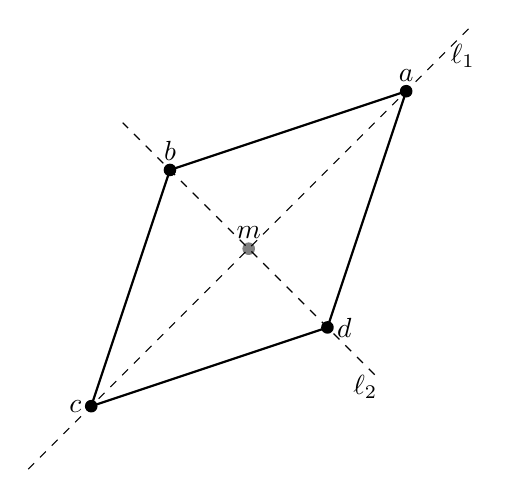
\begin{tikzpicture}[scale=1]

  \coordinate (A) at (0,0);
  \coordinate (B) at (3,1);
  \coordinate (C) at (4,4);
  \coordinate (D) at (1,3);
  \coordinate (E) at (2,2);

  \draw[thick] (A) -- (B) -- (C) -- (D) -- cycle;

  \node[left] at (A) {$c$};
  \node[right] at (B) {$d$};
  \node[above] at (C) {$a$};
  \node[above]  at (D) {$b$};
  \node[above]  at (E) {$m$};

  \fill (A) circle (0.08);
  \fill (B) circle (0.08);
  \fill (C) circle (0.08);
  \fill (D) circle (0.08);
  \fill[gray] (E) circle (0.08);


\path (A) -- (C) coordinate[pos=-0.2](A') coordinate[pos=1.2](C');
\draw[dashed] (A') -- (A) -- (C) -- (C')node[pos=0.9, below] {$\ell_1$};

\path (B) -- (D) coordinate[pos=-0.3](B') coordinate[pos=1.3](D');
\draw[dashed] (B') -- (B)node[pos=0.2, below] {$\ell_2$} -- (D) -- (D');

\end{tikzpicture}
\caption{A rhombus with center $m$ and diagonals $\ell_1,\ell_2$.}
\label{rhombusfigure}
\end{figure}
Let $L$ be the set of lines passing through at least two points of $P$ and let $$D:=\{(\ell_1,\ell_2)\in L^2\;|\;  \ell_1\perp \ell_2 \land |\ell_1\cap P|\geq |\ell_2\cap P|\}.$$
Further, let $R(P)$ denote the number of rhombi defined by $P$. For a line $\ell$ and point $x$, write $r_{\ell}(x):=|\{\{u,v\}\in \binom{\ell\cap P}{2}\;|\;u+v=2x\}|$. For two distinct non parallel lines $\ell_1$ and $\ell_2$, let $m_{\ell_1,\ell_2}$ denote the point of intersection of the two lines. Then
    $$R(P)\leq \sum_{\substack{(\ell_1,\ell_2)\in D }}r_{\ell_1}(m_{\ell_1,\ell_2})r_{\ell_2}(m_{\ell_1,\ell_2}).$$
Given $k\geq 1$, let $$R_k:=\sum_{\substack{(\ell_1,\ell_2)\in D\\  \\2^k\leq |\ell_1 \cap P|<2^{k+1}}}r_{\ell_1}(m_{\ell_1,\ell_2})r_{\ell_2}(m_{\ell_1,\ell_2}).$$
Put \(t=2^k\). First suppose that \(t\leq |P|^{1/2}\). By the Szemer\'{e}di-Trotter Theorem (Theorem~\ref{ST}), the number of lines \(\ell_1\in L\) satisfying
\(|\ell_1\cap P|\geq t\) is \(O(|P|^2/t^3)\). For a fixed such line
\(\ell_1\), every pair \(\{a,c\}\in \binom{\ell_1\cap P}{2}\)
determines the midpoint $m=(a+c)/2$, and hence determines the unique line \(\ell_2\) through \(m\) perpendicular
to \(\ell_1\). Since \((\ell_1,\ell_2)\in D\), we have $|\ell_2\cap P|\leq |\ell_1\cap P|<2t$, and therefore \(r_{\ell_2}(m)\leq 2t\). Thus



$$R_k\leq\sum_{\substack{\ell_1\in L\\ t\leq |\ell_1 \cap P|<2t}}\sum_{\{a,c\}\in{\binom{\ell_1\cap P}{2}}}r_{\ell_2}(m_{\ell_1,\ell_2})\ll \frac{|P|^2}{t^3} \binom{2t}{2}2t\ll |P|^2.$$
If $t> |P|^{1/2}$, then the number of lines $\ell_1\in L$ such that $|\ell_1\cap P|\geq t$ is at most $O(|P|/t)$. For fixed \(\ell_1\), every rhombus counted by \(R_k\) is determined by choosing one vertex
\(a\in \ell_1\cap P\) and one adjacent vertex
\(b\in P\setminus \ell_1\). Therefore,
$$R_k \ll\sum_{\substack{\ell_1\in L\\ t\leq |\ell_1 \cap P|<2t}}\sum_{a\in\ell_1\cap P}|P\setminus \ell_1|\leq \sum_{\substack{\ell_1\in L\\ t\leq |\ell_1 \cap P|<2t}} 2t |P|\ll |P|^2.$$
In total, the number of rhombi is 
\begin{align*}   
R(P)&\leq \sum_{\substack{(\ell_1,\ell_2)\in D }}r_{\ell_1}(m_{\ell_1,\ell_2})r_{\ell_2}(m_{\ell_1,\ell_2})
    =\sum_{k=1}^{\lceil \log_2|P| \rceil}\sum_{\substack{(\ell_1,\ell_2)\in D\\   \\2^k\leq |\ell_1 \cap P|<2^{k+1}}}r_{\ell_1}(m_{\ell_1,\ell_2})r_{\ell_2}(m_{\ell_1,\ell_2})  \\
    &=\sum_{k=1}^{\lceil \log_2|P| \rceil}R_k   
    \ll  |P|^2\log|P|,
    \end{align*}
completing the proof.
\end{proof}

\end{document}
